\documentclass[tikz]{standalone}
\begin{document}
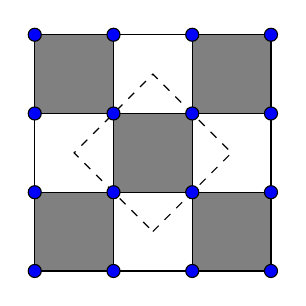
\begin{tikzpicture}

\fill [black!50] (0, 0)--(1, 0)--(1, 1)--(0, 1)--cycle;
%\draw [dotted] (0, 0)--(1, 1);
%\draw [dotted] (0, 1)--(1, 0);
\fill [black!50] (2, 0)--(3, 0)--(3, 1)--(2, 1)--cycle;
\fill [black!50] (1, 1)--(2, 1)--(2, 2)--(1, 2)--cycle;
\fill [black!50] (0, 2)--(1, 2)--(1, 3)--(0, 3)--cycle;
\fill [black!50] (2, 2)--(3, 2)--(3, 3)--(2, 3)--cycle;
\draw (0, 0)--(3, 0);
\draw (0, 1)--(3, 1);
\draw (0, 2)--(3, 2);
\draw (0, 3)--(3, 3);
\draw (0, 0)--(0, 3);
\draw (1, 0)--(1, 3);
\draw (2, 0)--(2, 3);
\draw (3, 0)--(3, 3);

\draw [dashed] (1.5, 0.5)--(2.5, 1.5)--(1.5, 2.5)--(0.5, 1.5)--cycle;

\draw (0, 0) node [circle, draw, fill=blue, scale=.5] {};
\draw (1, 0) node [circle, draw, fill=blue, scale=.5] {};
\draw (2, 0) node [circle, draw, fill=blue, scale=.5] {};
\draw (3, 0) node [circle, draw, fill=blue, scale=.5] {};

\draw (0, 1) node [circle, draw, fill=blue, scale=.5] {};
\draw (1, 1) node [circle, draw, fill=blue, scale=.5] {};
\draw (2, 1) node [circle, draw, fill=blue, scale=.5] {};
\draw (3, 1) node [circle, draw, fill=blue, scale=.5] {};

\draw (0, 2) node [circle, draw, fill=blue, scale=.5] {};
\draw (1, 2) node [circle, draw, fill=blue, scale=.5] {};
\draw (2, 2) node [circle, draw, fill=blue, scale=.5] {};
\draw (3, 2) node [circle, draw, fill=blue, scale=.5] {};

\draw (0, 3) node [circle, draw, fill=blue, scale=.5] {};
\draw (1, 3) node [circle, draw, fill=blue, scale=.5] {};
\draw (2, 3) node [circle, draw, fill=blue, scale=.5] {};
\draw (3, 3) node [circle, draw, fill=blue, scale=.5] {};
\end{tikzpicture}
\end{document}
